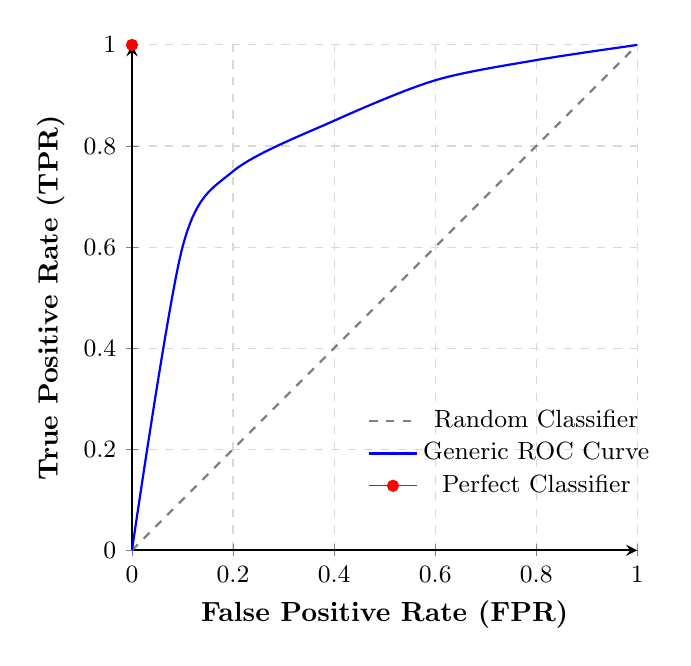
\begin{tikzpicture}
    \begin{axis}[
      width=8cm, height=8cm,
      grid=both, % Adds grid
      grid style={dashed, gray!30},
      xlabel={False Positive Rate (FPR)},
      ylabel={True Positive Rate (TPR)},
      xmin=0, xmax=1, % Limits for x-axis (FPR)
      ymin=0, ymax=1, % Limits for y-axis (TPR)
      axis lines=left,
      axis line style={thick},
      label style={font=\bfseries},
      tick label style={font=\small},
      xtick={0,0.2,0.4,0.6,0.8,1}, % X-axis ticks
      ytick={0,0.2,0.4,0.6,0.8,1}, % Y-axis ticks
      legend style={at={(0.45,0.3)},anchor=north west,draw=none,fill=none, font=\small}
    ]
  
    % Plotting the random classifier (diagonal)
    \addplot[domain=0:1, thick, dashed, gray] {x};
    \addlegendentry{Random Classifier}
  
    % Plotting the ROC curve for a typical classifier
    \addplot[thick, smooth, blue] coordinates {
      (0,0) (0.1,0.6) (0.2,0.75) (0.4,0.85) (0.6,0.93) (0.8,0.97) (1,1)
    };
    \addlegendentry{Generic ROC Curve}
  
    % Highlighting the perfect point (0,1)
    \addplot[mark=*, mark size=2pt, color=red] coordinates {(0,1)};
    \node[above right] at (axis cs: 0,1) {};
    \addlegendentry{Perfect Classifier}
  
    \end{axis}
  \end{tikzpicture}